\section{分层采样}\label{sec:分层采样}
我们将要介绍的首个\refvar{Sampler}{}实现会把
像素区域细分为矩形区域并在每个区域内生成单个样本。
这些区域常称为\keyindex{层}{strata}{},
而该采样器称为\refvar{StratifiedSampler}{}。
分层背后的关键思想是通过把采样域细分为不重叠区域
并从每个中取单个样本,我们更不可能错失整个图像的重要特征,
因为保证了样本不会全都挨在一起。换句话说,
如果许多样本都从样本空间中的邻近点取得则对我们没有好处,
因为每个新样本不能增加许多关于图像函数特性的新信息。
从信号处理的角度看,我们在隐式定义整体采样率,
它使得层级越小,我们拥有的层数就越多,因此采样率就越高。

分层采样器通过对层中心点施加一个至多为层的一半宽高的
随机\keyindex{扰动}{jitter}{}量来将每个样本置于每层中的随机点处。
如\refsec{采样理论}讨论的,该扰动引起的非均匀性帮助把混叠转化为噪声。
采样器还提供了非扰动模式,给出层中的均匀采样;
比起用于渲染高质量图像,该模式对于比较不同采样技术才最有用。

直接对高维采样应用分层法很快导致样本量巨大。
例如,如果我们在每个维度上把5D的图像、透镜和时间样本空间划分为四层,
则每个像素的样本总量将是$4^5=1024$.
我们可以通过在某些维度取更少的样本(或者不分层某些维度,实际上使用单层)来降低该影响,
但我们将会失去在这些维度拥有分层良好的样本的好处。
该分层问题称为\keyindex{维度灾难}{curse of dimensionality}{}。

通过为域的维度子集计算低维分层模式然后随机联合每个维度集合中的样本,
我们可以获取分层的大多数好处而不用为过多采样总量付出代价
(该过程有时称为\keyindex{填充}{padding}{})。
\reffig{7.16}展示了基本思想:我们可能只想每个像素取四个样本,
但仍得在所有维度上对样本分层。我们独立生成四个2D分层图像样本,
四个1D分层时间样本,以及四个2D分层透镜样本。
然后我们随机地为每个图像样本联合一个时间以及透镜样本值。
结果是每个像素拥有合起来良好覆盖样本空间的样本。
\begin{figure}[htbp]
    \centering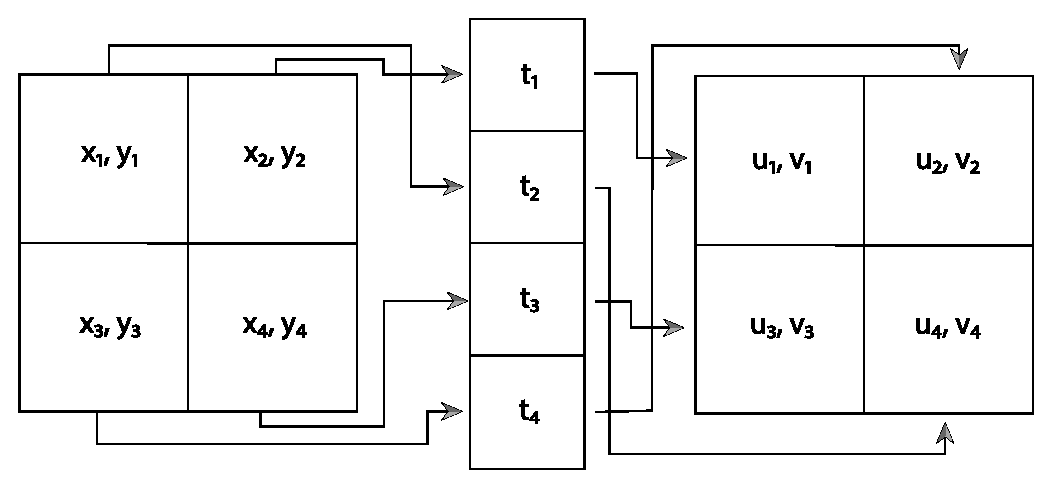
\includegraphics[width=0.8\linewidth]{chap07/Samplepadding.eps}
    \caption{我们可以生成良好的样本模式并获得分层的好处而不要求
        同时对所有采样维度分层。这里,我们已把$(x,y)$图像位置、
        时间$t$以及$(u,v)$透镜位置分为独立的层,每个都有四个区域。
        每个都是独立采样的,然后每个图像样本都随机关联一个时间样本
        和一个透镜样本。我们保留了在每个单独维度上分层的好处而不用指数级地增加样本总量。}
    \label{fig:7.16}
\end{figure}

\reffig{7.17}展示了在渲染景深时使用分层的透镜样本和
使用不分层的随机样本相比图像质量的提升。
\begin{figure}[htbp]
    \subfloat[参考]{
\includegraphics[width=0.49\linewidth]{chap07/dof-ref.png}\label{fig:7.17.1}}\,
    \subfloat[随机采样]{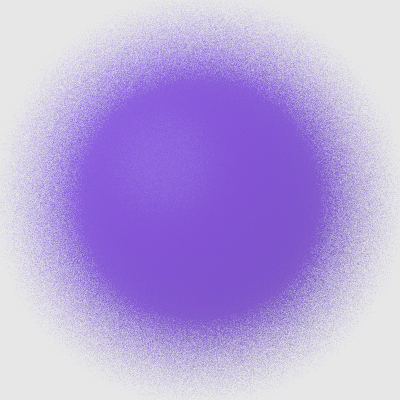
\includegraphics[width=0.49\linewidth]{chap07/dof-random.png}\label{fig:7.17.2}}\\
    \subfloat[分层采样]{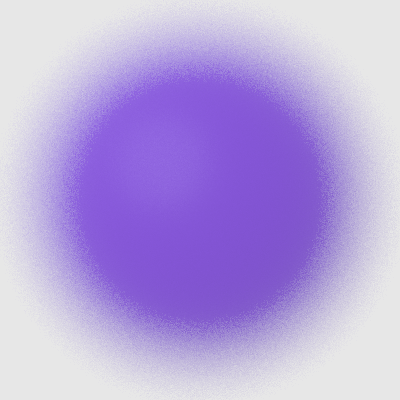
\includegraphics[width=0.49\linewidth]{chap07/dof-stratified.png}\label{fig:7.17.3}}
    \caption{渲染有景深的紫色球体时采样模式的影响。
        (a)模糊球体的高质量参考图像。(b)在每个像素中随机采样而无分层所生成的图像。
        (c)用同样数量的样本生成的图像,但用的是\refvar{StratifiedSampler}{},
        它分层了图像样本以及对该图更重要的透镜样本。对于该情形分层法做出了很大改善。}
    \label{fig:7.17}
\end{figure}

\reffig{7.18}展示比较了几种采样模式。
第一种是完全随机的模式:我们生成大量样本而完全不使用分层。
其结果很差;一些区域只有几个样本而另一些区域有好几团样本。
第二种是均匀分层模式。最后,均匀模式被扰动,
随机偏移量被加到每个样本的位置上,但仍将其保留在格子中。
这给出了比纯随机模式更好的整体分布而又保留了分层的好处,
尽管仍有一些样本团以及欠采样的区域。
\begin{figure}[htbp]
    \subfloat[]{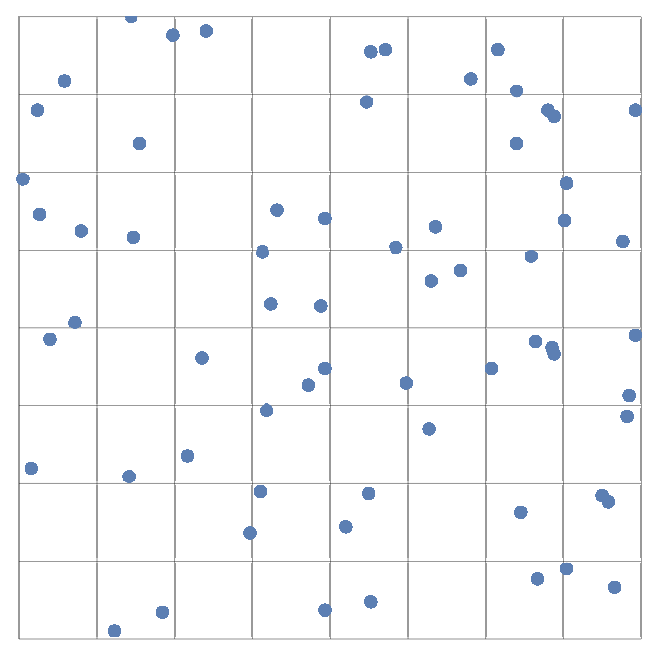
\includegraphics[width=0.49\linewidth]{chap07/random-point-samples.eps}\label{fig:7.18.1}}\,
    \subfloat[]{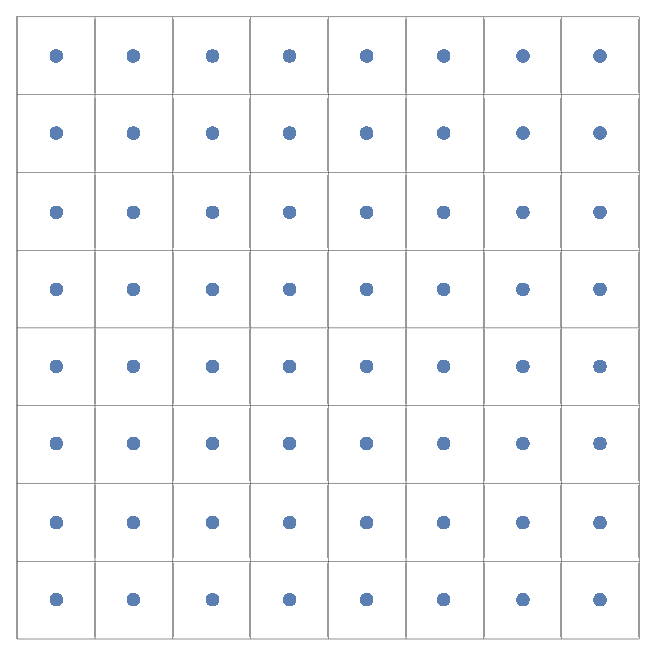
\includegraphics[width=0.49\linewidth]{chap07/uniform-point-samples.eps}\label{fig:7.18.2}}\\
    \subfloat[]{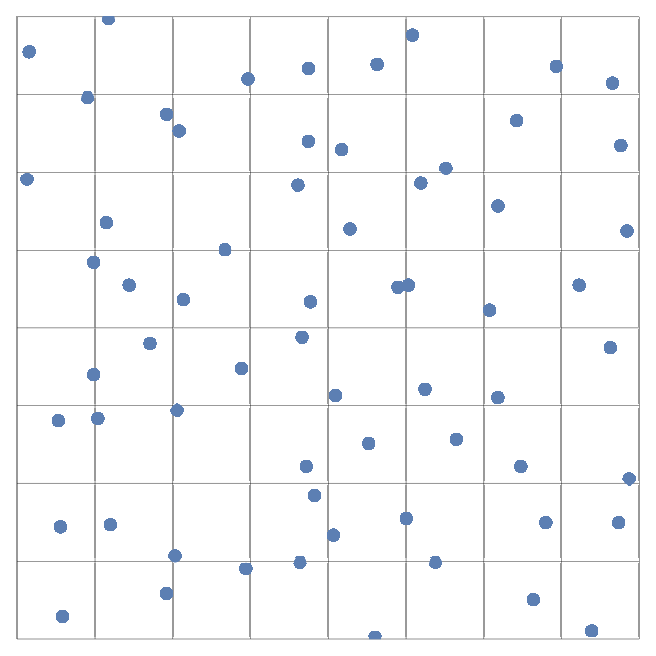
\includegraphics[width=0.49\linewidth]{chap07/jittered-point-samples.eps}\label{fig:7.18.3}}
    \caption{三种2D采样模式。(a)随机模式是无效模式,许多样本团让大片图像没有好好采样。
        (b)均匀分层模式的分布更好但会加剧混叠伪影。
        (c)分层扰动模式将来自均匀模式的混叠转化为高频噪声而仍保留了分层的好处。}
    \label{fig:7.18}
\end{figure}

\reffig{7.19}展示了用\refvar{StratifiedSampler}{}渲染的图像,
并展示了扰动的样本位置怎样将混叠伪影转化为不那么讨厌的噪声。
\begin{figure}[htbp]
    \centering
    \subfloat[参考]{\includegraphics[width=0.8\linewidth]{chap07/checkerboard-ref.png}\label{fig:7.19.1}}\\
    \subfloat[1个均匀样本]{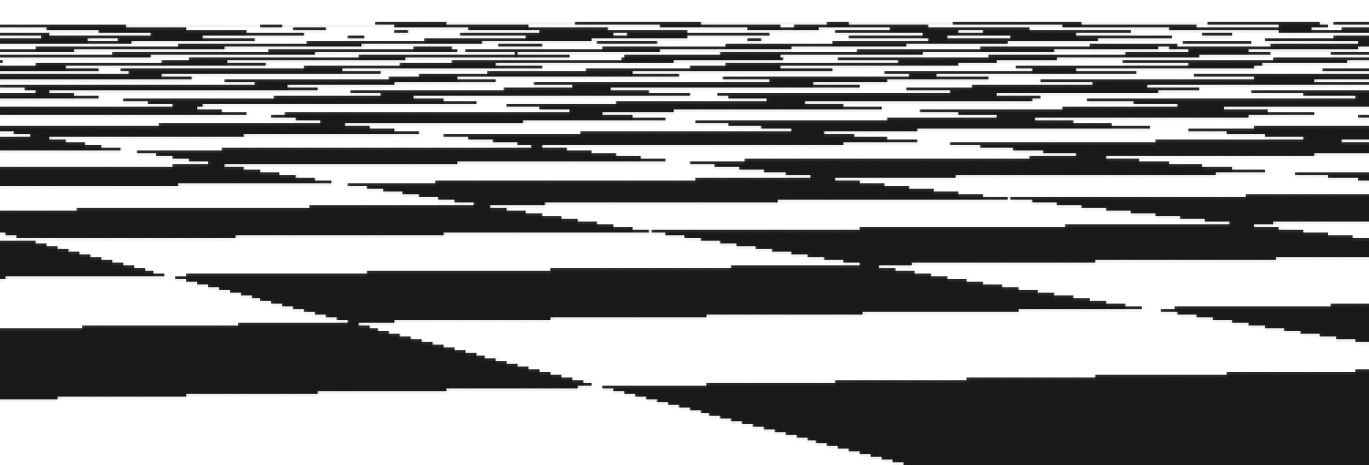
\includegraphics[width=0.8\linewidth]{chap07/checkerboard-unif-1spp.png}\label{fig:7.19.2}}\\
    \subfloat[1个扰动样本]{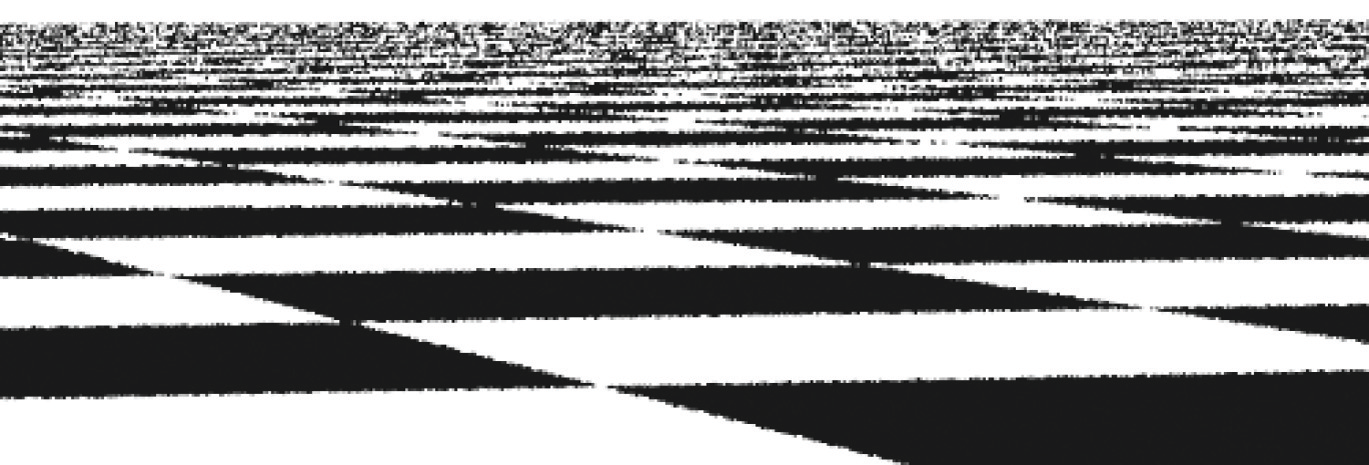
\includegraphics[width=0.8\linewidth]{chap07/checkerboard-jitter-1spp.png}\label{fig:7.19.3}}\\
    \subfloat[4个扰动样本]{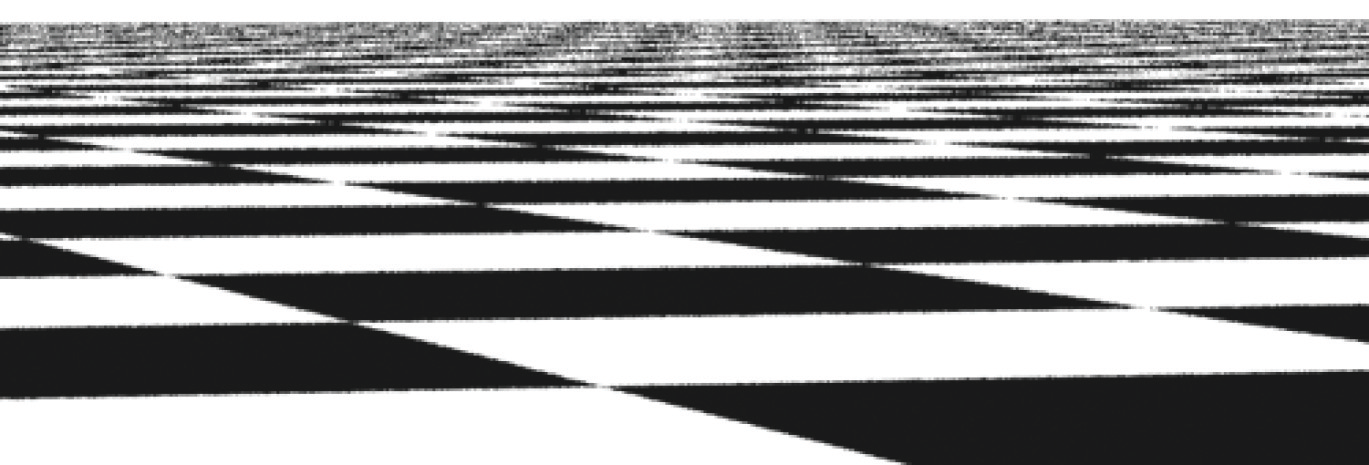
\includegraphics[width=0.8\linewidth]{chap07/checkerboard-jitter-4spp.png}\label{fig:7.19.4}}
    \caption{用棋盘纹理比较图像采样方法。这是幅很难渲染好的图像,
        因为当我们接近地平线时棋盘格关于像素间隔的频率趋于无穷。
        (a)参考图像,每个像素用256个样本渲染,展示了接近理想结果的样子。
        (b)每个像素只用一个样本渲染的图像,没有扰动。注意前景中格子边缘的锯齿伪影。
        还注意棋盘格函数在样本之间经历了许多周期的距离处的伪影;
        如之前介绍过的信号处理理论所料,细节错误地重复表现为低频混叠。
        (c)扰动图像样本的结果,每个像素还是只有一个样本。
        第二幅图像规则的混叠已经被替换为不那么讨厌的噪声伪影。
        (d)每个像素用四个扰动样本的结果仍然不如参考图像,但明显优于之前的结果。}
    \label{fig:7.19}
\end{figure}

\begin{lstlisting}
`\initcode{StratifiedSampler Declarations}{=}`
class `\initvar{StratifiedSampler}{}` : public `\refvar{PixelSampler}{}` {
public:
    `\refcode{StratifiedSampler Public Methods}{}`
private:
    `\refcode{StratifiedSampler Private Data}{}`
};
\end{lstlisting}
\begin{lstlisting}
`\initcode{StratifiedSampler Public Methods}{=}`
`\refvar{StratifiedSampler}{}`(int xPixelSamples, int yPixelSamples,
        bool jitterSamples, int nSampledDimensions)
    : `\refvar{PixelSampler}{}`(xPixelSamples * yPixelSamples, nSampledDimensions),
      `\refvar{xPixelSamples}{}`(xPixelSamples), `\refvar{yPixelSamples}{}`(yPixelSamples),
      `\refvar{jitterSamples}{}`(jitterSamples) { }
\end{lstlisting}
\begin{lstlisting}
`\initcode{StratifiedSampler Private Data}{=}`
const int `\initvar{xPixelSamples}{}`, `\initvar{yPixelSamples}{}`;
const bool `\initvar{jitterSamples}{}`;
\end{lstlisting}

作为\refvar{PixelSampler}{}的子类,
\refvar[StratifiedSampler::StartPixel]{StartPixel}{()}的实现必须按照传给\refvar{PixelSampler}{}
构造函数的维数{\ttfamily nSampledDimensions}一起生成1D和2D样本以及请求的数组样本。
\begin{lstlisting}
`\initcode{StratifiedSampler Method Definitions}{=}`
void `\refvar{StratifiedSampler}{}`::`\initvar[StratifiedSampler::StartPixel]{StartPixel}{}`(const `\refvar{Point2i}{}` &p) {
    `\refcode{Generate single stratified samples for the pixel}{}`
    `\refcode{Generate arrays of stratified samples for the pixel}{}`
    `\refvar{PixelSampler}{}`::StartPixel(p);
}
\end{lstlisting}

生成初始的分层样本后,它们被随机打乱;这是本节开头描述的填充方法。
如果没有进行打乱,则样本维度的值可能以某种方式相关而引发图像中的错误——
例如,用于选择胶片位置的首个2D样本和首个2D透镜样本会总是都在相邻于原点的左下方那层。
\begin{lstlisting}
`\initcode{Generate single stratified samples for the pixel}{=}`
for (size_t i = 0; i < `\refvar{samples1D}{}`.size(); ++i) {
    `\refvar{StratifiedSample1D}{}`(&`\refvar{samples1D}{}`[i][0], `\refvar{xPixelSamples}{}` * `\refvar{yPixelSamples}{}`,
                       `\refvar[PixelSampler::rng]{rng}{}`, `\refvar{jitterSamples}{}`);
    `\refvar{Shuffle}{}`(&`\refvar{samples1D}{}`[i][0], `\refvar{xPixelSamples}{}` * `\refvar{yPixelSamples}{}`, 1, `\refvar[PixelSampler::rng]{rng}{}`);
}
for (size_t i = 0; i < `\refvar{samples2D}{}`.size(); ++i) {
    `\refvar{StratifiedSample2D}{}`(&`\refvar{samples2D}{}`[i][0], `\refvar{xPixelSamples}{}`, `\refvar{yPixelSamples}{}`,
                       `\refvar[PixelSampler::rng]{rng}{}`, `\refvar{jitterSamples}{}`);
    `\refvar{Shuffle}{}`(&`\refvar{samples2D}{}`[i][0], `\refvar{xPixelSamples}{}` * `\refvar{yPixelSamples}{}`, 1, `\refvar[PixelSampler::rng]{rng}{}`);
}
\end{lstlisting}

1D和2D分层采样例程实现为实用函数。
两个都在域中给定层数上循环并在每个里面放置一个样本点。
\begin{lstlisting}
`\initcode{Sampling Function Definitions}{=}\initnext{SamplingFunctionDefinitions}`
void `\initvar{StratifiedSample1D}{}`(`\refvar{Float}{}` *samp, int nSamples, `\refvar{RNG}{}` &rng,
        bool jitter) {
    `\refvar{Float}{}` invNSamples = (`\refvar{Float}{}`)1 / nSamples;
    for (int i = 0; i < nSamples; ++i) {
        `\refvar{Float}{}` delta = jitter ? rng.`\refvar{UniformFloat}{}`() : 0.5f;
        samp[i] = std::min((i + delta) * invNSamples, `\refvar{OneMinusEpsilon}{}`);
    }
}
\end{lstlisting}

\refvar{StratifiedSample2D}{()}同样生成范围$[0,1)^2$中的样本。
\begin{lstlisting}
`\refcode{Sampling Function Definitions}{+=}\lastnext{SamplingFunctionDefinitions}`
void `\initvar{StratifiedSample2D}{}`(`\refvar{Point2f}{}` *samp, int nx, int ny, `\refvar{RNG}{}` &rng,
        bool jitter) {
    `\refvar{Float}{}` dx = (`\refvar{Float}{}`)1 / nx, dy = (`\refvar{Float}{}`)1 / ny;
    for (int y = 0; y < ny; ++y)
        for (int x = 0; x < nx; ++x) {
            `\refvar{Float}{}` jx = jitter ? rng.`\refvar{UniformFloat}{}`() : 0.5f;
            `\refvar{Float}{}` jy = jitter ? rng.`\refvar{UniformFloat}{}`() : 0.5f;
            samp->x = std::min((x + jx) * dx, `\refvar{OneMinusEpsilon}{}`);
            samp->y = std::min((y + jy) * dy, `\refvar{OneMinusEpsilon}{}`);
            ++samp;
        }
}
\end{lstlisting}

函数\refvar{Shuffle}{()}随机重排含有{\ttfamily count}个样本值的数组,
每个都有{\ttfamily nDimensions}维(换句话说,
尺寸为{\ttfamily nDimensions}的值构成的块被重排)。
\begin{lstlisting}
`\initcode{Sampling Inline Functions}{=}\initnext{SamplingInlineFunctions}`
template <typename T>
void `\initvar{Shuffle}{}`(T *samp, int count, int nDimensions, `\refvar{RNG}{}` &rng) {
    for (int i = 0; i < count; ++i) {
        int other = i + rng.`\refvar{UniformUInt32}{}`(count - i);
        for (int j = 0; j < nDimensions; ++j)
            std::swap(samp[nDimensions * i + j],
                      samp[nDimensions * other + j]);
    }
}
\end{lstlisting}

样本数组给我们出了个难题:例如若一个积分器
为像素中的每个样本请求样本向量中含64个2D样本值的数组,
则采样器有两个不同的目标要达成:
\begin{enumerate}
    \item 希望数组内的样本本身在2D上分布良好(例如通过使用$8\times8$分层网格)。
          这里的分层法会为每个单独的样本向量提升算出的结果的质量。
    \item 最好保证一个图像样本的数组中的每个样本都不要和图像中相邻样本的任何样本值太相似。
          即我们更希望点相对于其邻居能分布良好,使得在单个像素周围区域上就能很好覆盖整个样本空间。
\end{enumerate}

比起尝试同时解决这里的两个问题,\refvar{StratifiedSampler}{}只解决第一个。
本章后面的其他采样器会以更加精巧的技术回顾该问题并在不同程度上同时解决它们。

第二个复杂性来自于调用者可能会为每个图像样本请求任意数量样本的事实,
所以可能不易应用分层法。(例如,我们要怎么生成七个样本的分层2D模式?)
我们只能生成一个$n\times1$或$1\times n$的分层模式,
但这只能给我们在一个维度上分层的好处但不保证其他维度有好的模式。
方法{\ttfamily StratifiedSampler::RoundSize()}可以将请求进位到
下一个平方数,但我们将换用一种称为\keyindex{拉丁超立方采样}{Latin hypercube sampling}{}(LHS)的方法,
它能生成具有相当好分布的任意数量的任意维数样本。

LHS把每个维度轴均匀划分为$n$个区域并沿对角线在$n$个区域中的
每一个内生成一个扰动的样本,如\reffig{7.20}左边所示。
然后这些样本在每个维度上被随机打乱,生成分布良好的模式。
\begin{figure}[htbp]
    \centering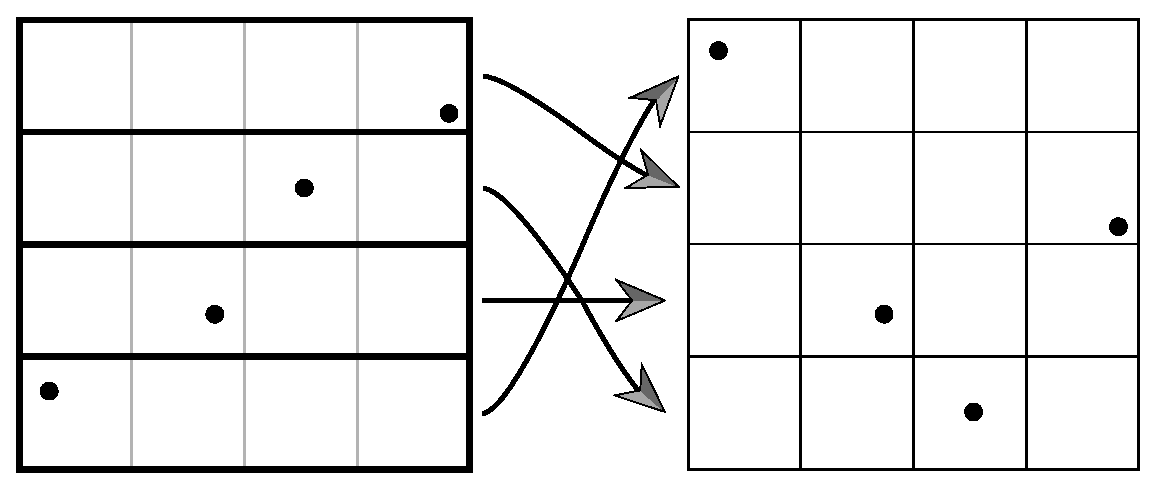
\includegraphics[width=0.8\linewidth]{chap07/LHSshuffle.eps}
    \caption{拉丁超立方采样(有时称为\protect\keyindex{$n$车采样}{$n$-rooks sampling}{})
        选择样本使得网格每行每列只出现单个样本。通过在对角线格子里生成随机样本
        然后随机重排它们的坐标可以做到这点。LHS的一个优点是它能像用分层模式那样
        生成具有良好分布的任意数量的样本,而不仅仅是$m\times n$个样本。}
    \label{fig:7.20}
\end{figure}

LHS的一个优点是当样本投影到样本维度的任意轴时它最小化了样本的聚集。
该性质与分层采样相反,后者2D模式中$n\times n$个样本里的$2n$个可能投影到每个轴上基本相同的点。
\reffig{7.21}展示了对于分层采样模式的这一最坏情况。
\begin{figure}[htbp]
    \centering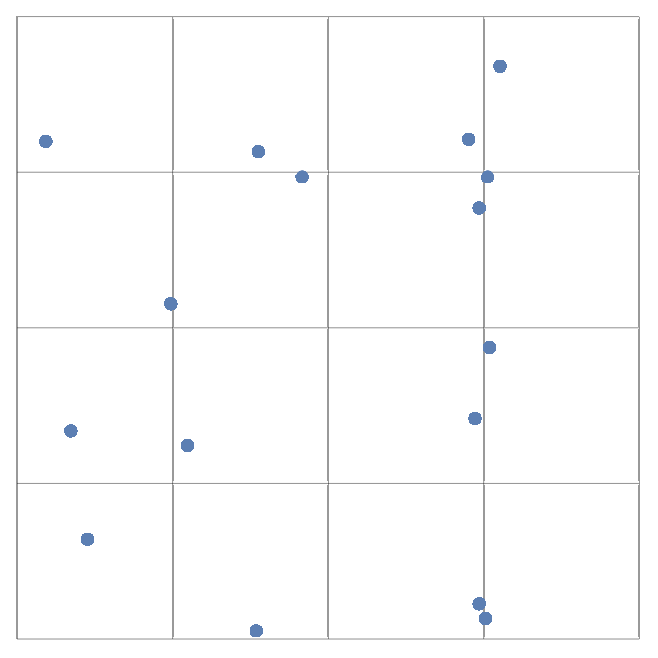
\includegraphics[width=0.4\linewidth]{chap07/stratified-bad-luck.eps}
    \caption{分层采样的一个最坏情况。在$n\times n$的2D模式中,
        多达$2n$个点可能投影到一个轴上基本相同的点。当生成像这样的“倒霉”模式时,
        用其算出的结果质量通常堪忧(这里,8个样本有几乎一样的$x$值)。}
    \label{fig:7.21}
\end{figure}

尽管解决了聚集问题,LHS对于分层采样并不是必要的改进;
很容易构造样本位置基本共线且大面积采样域没有相邻样本的情形
(例如原始样本的排列一致的时候,即让它们都保持原样)。
特别地,随着$n$增加,拉丁超立方模式比起分层模式越来越低效
\footnote{后续章节我们将回顾该问题,讨论同时是分层的且按拉丁超立方模式分布的样本模式。}。

通用的函数\refvar{LatinHypercube}{()}在任意维度生成任意数量的LHS样本。
因此数组{\ttfamily samples}中的元素数量应为{\ttfamily nSamples*nDim}。

\begin{lstlisting}
`\refcode{Sampling Function Definitions}{+=}\lastnext{SamplingFunctionDefinitions}`
void `\initvar{LatinHypercube}{}`(`\refvar{Float}{}` *samples, int nSamples, int nDim, `\refvar{RNG}{}` &rng) {
    `\refcode{Generate LHS samples along diagonal}{}`
    `\refcode{Permute LHS samples in each dimension}{}`
}
\end{lstlisting}
\begin{lstlisting}
`\initcode{Generate LHS samples along diagonal}{=}`
`\refvar{Float}{}` invNSamples = (`\refvar{Float}{}`)1 / nSamples;
for (int i = 0; i < nSamples; ++i)
    for (int j = 0; j < nDim; ++j) {
        `\refvar{Float}{}` sj = (i + (rng.`\refvar{UniformFloat}{}`())) * invNSamples;
        samples[nDim * i + j] = std::min(sj, `\refvar{OneMinusEpsilon}{}`);
    }
\end{lstlisting}

为了进行重排,该函数在样本上循环,每次在一个维度上随机重排样本点。
注意这和之前的\refvar{Shuffle}{()}例程是不一样的重排:
后者例程做一次重排,每个样本里的全部{\ttfamily nDim}个样本点是保持在一起的,
而这里是{\ttfamily nDim}次对单个维度的依次单独重排(\reffig{7.22})
\footnote{尽管不需要重排LHS模式的第一维,但这里的实现还是这样做了,
    因为让第一维的元素变为随机顺序意味着LHS模式可以与来自其他源的采样模式
    结合使用而没有其样本点间存在相关性的危险。}。
\begin{figure}[htbp]
    \centering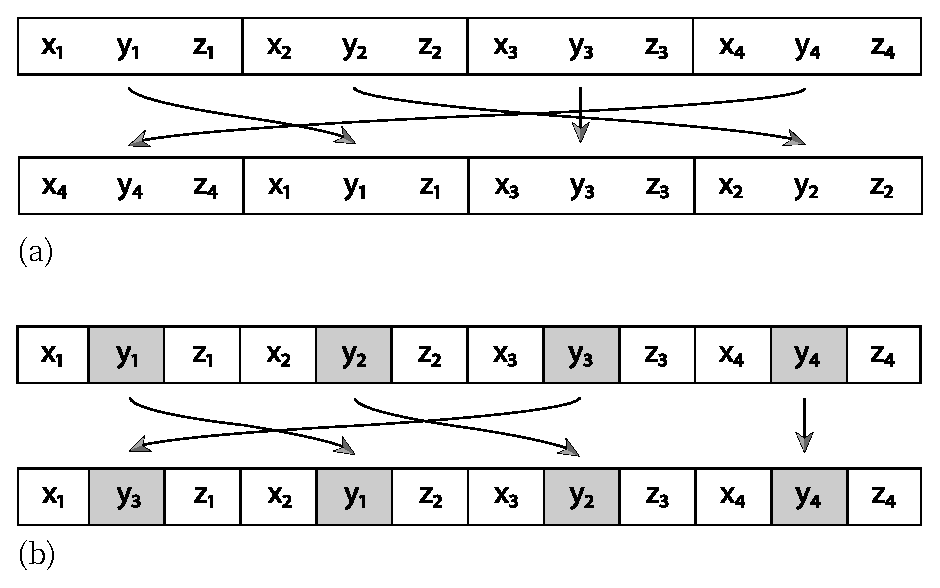
\includegraphics[width=0.8\linewidth]{chap07/Shufflepermutations.eps}
    \caption{(a)\refvar{Shuffle}{()}例程进行的重排移动附近的整块元素。
        (b)拉丁超立方采样的重排独立地排列每个维度的样本。
        这里展示了打乱四个三维元素模式的第二维样本。}
    \label{fig:7.22}
\end{figure}

\begin{lstlisting}
`\initcode{Permute LHS samples in each dimension}{=}`
for (int i = 0; i < nDim; ++i) {
    for (int j = 0; j < nSamples; ++j) {
        int other = j + rng.`\refvar{UniformUInt32}{}`(nSamples - j);
        std::swap(samples[nDim * j + i], samples[nDim * other + i]);
    }
}
\end{lstlisting}

有了函数\refvar{LatinHypercube}{()},
我们现在可以编写代码为当前像素计算样本数组了。
1D样本被分层然后随机打乱,而2D样本用拉丁超立方采样生成。
\begin{lstlisting}
`\initcode{Generate arrays of stratified samples for the pixel}{=}`
for (size_t i = 0; i < `\refvar{samples1DArraySizes}{}`.size(); ++i)
    for (int64_t j = 0; j < `\refvar{samplesPerPixel}{}`; ++j) {
        int count = `\refvar{samples1DArraySizes}{}`[i];
        `\refvar{StratifiedSample1D}{}`(&`\refvar{sampleArray1D}{}`[i][j * count], count, `\refvar[PixelSampler::rng]{rng}{}`,
                           `\refvar{jitterSamples}{}`);
        `\refvar{Shuffle}{}`(&`\refvar{sampleArray1D}{}`[i][j * count], count, 1, `\refvar[PixelSampler::rng]{rng}{}`);
    }
for (size_t i = 0; i < `\refvar{samples2DArraySizes}{}`.size(); ++i)
    for (int64_t j = 0; j < `\refvar{samplesPerPixel}{}`; ++j) {
        int count = `\refvar{samples2DArraySizes}{}`[i];
        `\refvar{LatinHypercube}{}`(&`\refvar{sampleArray2D}{}`[i][j * count].x, count, 2, `\refvar[PixelSampler::rng]{rng}{}`);
    }
\end{lstlisting}

我们将用\reffig{7.23}中的场景来阐述一些\refvar{Sampler}{}实现的性质。
\begin{figure}[htbp]
    \centering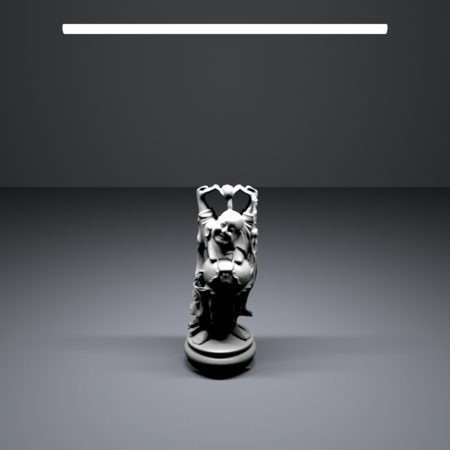
\includegraphics[width=0.75\linewidth]{chap07/area-light-example.png}
    \caption{面光源采样示例场景。}
    \label{fig:7.23}
\end{figure}

\reffig{7.24}展示了对于\refvar{DirectLightingIntegrator}{}而言来自好样本的提升。
第一幅图像每个像素用1个图像样本算得,每个有16个阴影样本。
第二幅每个像素用16个图像样本,每个有1个阴影样本。
因为\refvar{StratifiedSampler}{}能为第一种情况生成良好的LHS模式,
所以即使在取用的阴影样本总数相同时,其阴影质量也好得多。

\begin{figure}[htbp]
    \centering
    \subfloat[1个图像样本,16个阴影样本]{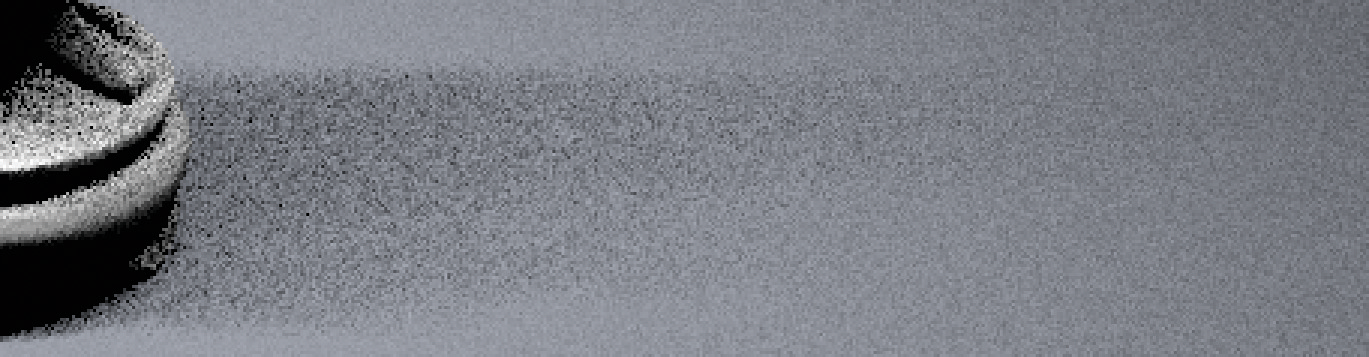
\includegraphics[width=\linewidth]{chap07/shadow-1-16.png}\label{fig:7.24.1}}\\
    \subfloat[16个图像样本,1个阴影样本]{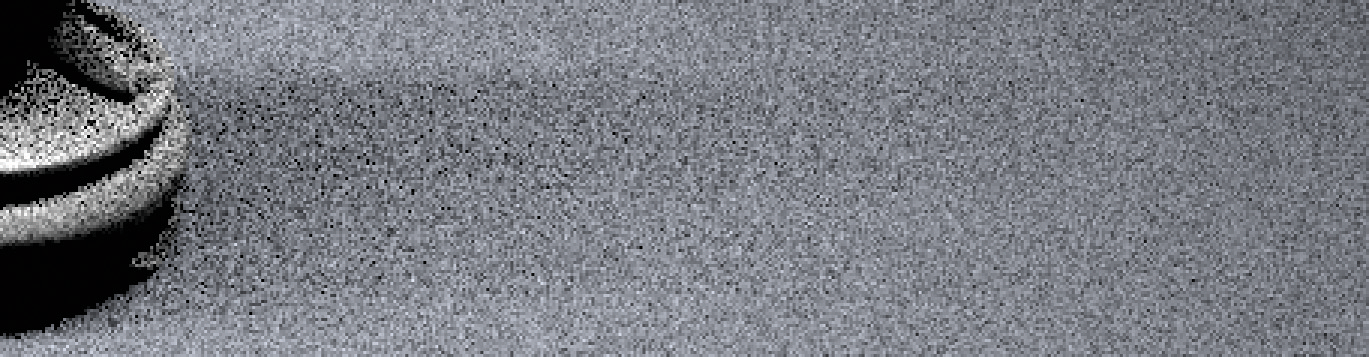
\includegraphics[width=\linewidth]{chap07/shadow-16-1.png}\label{fig:7.24.2}}
    \caption{用来自分层采样器的样本采样面光源。
        (a)展示了每个像素用1个图像样本和16个阴影样本的结果,
        而(b)展示了用16个图像样本且每个只有1个阴影样本的结果。
        两种情况阴影样本的总数是一样的,但因为每个图像样本用16个阴影样本的版本
        可以使用LHS模式,像素区域内所有阴影样本都良好分布,而第二幅图像里
        这里的实现没有办法防止它们分布得很差。差别是惊人的。}
    \label{fig:7.24}
\end{figure}